\subsection{Kernel Treiber}

\dirtree{%
.1 ROOT.
.2 Level 2.
.2 Correct format e.g.~DD.MM.YYYY. %% or e.g.\ DD.MM.YYYY.
}

\subsubsection{Temperatursensor über \acrshort{i2c}}

\Gls{i2c} Adapter Initialisieren.
\lstinputlisting[firstnumber=17, firstline=17,lastline=27, title=./driver/src/temp.c]{../../driver/src/temp.c}

\Gls{i2c} Adapter De-initialisieren.
\lstinputlisting[firstnumber=29, firstline=29,lastline=34, title=./driver/src/temp.c]{../../driver/src/temp.c}

Der \texttt{TMP102} Sensor gibt Messdaten mit 13-Bit Präzision bei einer Auflösung von $0.0625\si{\degree C}$ am \gls{lsb} an.
Um einen Messwert zu einer Temperatur zu konvertieren müssen zuerst zwei Byte gelesen werden.
Diese müssen zu einem 16-Bit Wert, welcher den ogrinellen 13-Bit Messwert beinhaltet, konkatiniert werden.
Anschlie{\ss}end muss der Messwert linear abgebildet werden, dass hei{\ss}t mit der Auflösung pro \gls{lsb} multiplizieren.
Die \gls{fpu} sollte unter allen Umständen nicht aus dem Kernelspace verwendet werden,
da die Kontextänderung abträgliche Performanceimplikationen auf Userspace Applikationen mit sich führen kann.
Die berechnung wird folglich mit der Integerdivision des Kehrwerts wie in \autoref{eq:temp-convert} ausgeführt.
Der Fehler der Berechnung wird in \autoref{eq:temp-error} aufgeführt und in \autoref{fig:rounding-err} visualisiert.
Der resultierende Rundungsfehler manifestiert sich als Rauschen.
Da unsere Anwednung sich nominal bei und über Raumtemperatur in Einer-Stellen Präzision agiert sind die resultierenden Fehler vernachlässigbar.

\begin{equation}
    \vartheta = \texttt{M}_D \cdot 0.0625\si{\celsius} = \frac{\texttt{M}_D}{\left(0.0625\si{\celsius}\right)^{-1}} = \frac{\texttt{M}_D}{16\si{\per\celsius}} \approx \left\lfloor\frac{\texttt{M}_D}{16\si{\per\celsius}}\right\rfloor
    \label{eq:temp-convert}
\end{equation}
\begin{equation}
    \begin{aligned}
        \Delta_{\texttt{M}_D} &= \frac{\texttt{M}_D}{16\si{\celsius}} - \left\lfloor\frac{\texttt{M}_D}{16\si{\per\celsius}}\right\rfloor \\[2ex]
        \delta_{\texttt{M}_D} &= \frac{\Delta_{\texttt{M}_D}}{\frac{\texttt{M}_D}{16\si{\celsius}} } \\[2ex]
    \end{aligned}
    \label{eq:temp-error}
\end{equation}
\begin{figure}
    \centering
    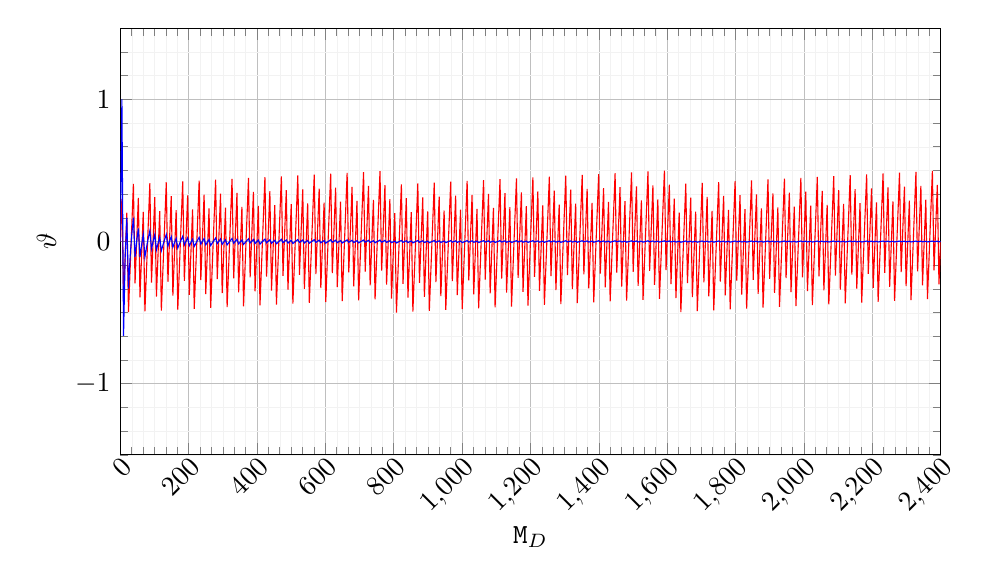
\begin{tikzpicture}
        \begin{axis}[%
            xmin=0,
            xmax=2400,
            ymin=-1.5,
            ymax=1.5,
            samples=500,
            width=12cm,
            height=7cm,
            minor tick num=5,
            grid=both,
            grid style={line width=.1pt, draw=gray!10},
            major grid style={line width=.2pt,draw=gray!50},
            % nodes near coords,
            xlabel near ticks,
            xticklabel style={rotate=45,anchor=north east,inner sep=0mm},
            xlabel={$\texttt{M}_D$},
            ylabel={$\vartheta$},
            ylabel near ticks]
            % \addplot[domain=0:6.4, blue, very thick, smooth, ->] {2.1971*1.8206^x};
            \addplot[domain=0:2400, red] {(x * 0.0625) - round(x / 16)};
            \addplot[domain=0:2400, blue] {((x * 0.0625) - round(x / 16)) / (x * 0.0625)};
        \end{axis}
    \end{tikzpicture}
    \caption[Integerdivisionsinduzierter Rundungsfehler]{Integerdivisionsinduzierter Rundungsfehler der Temperatursensorkonversion
    \textcolor{red}{Rot: Absoluter Fehler $\Delta_{\texttt{M}_D}$.}
    \textcolor{blue}{Blau: Relativer Fehler $\delta_{\texttt{M}_D}$.}
    }
    \label{fig:rounding-err}
\end{figure}
\lstinputlisting[firstnumber=37, firstline=37,lastline=49, title=./driver/src/temp.c]{../../driver/src/temp.c}

\subsubsection{Potentiometer über \acrshort{spi}}

\subsubsubsection{Protokoll}

\subsubsubsection{Softwareablauf}

\subsubsubsection{Devicetree Overlay}
Auf dem \gls{rpi} muss der \gls{spi} Treiber durch \texttt{raspi-config} aktiviert werden.
Dadurch werden unter \texttt{/dev} zwei \gls{spi} Treiber angelegt und das Hardware \gls{spi} Subsystem aktiviert.
Die angelegten Treiber stellen eine \gls{api}-Verbindung zwischen Kernelspace und der Hardware dar.
Jedoch werden durch die Treiber die \gls{ss} Signale belegt.
Der Treiber zur Kommunikation über \gls{spi} funktioniert, kann jedoch aufgrund dessen nicht durch externe Programme im Kernelspace beansprucht werden.
Um dies zu umgehen muss der Zugriff auf die \gls{ss} Signale durch die durch das System bereitgestellten Treiber unterbunden werden.

Dazu wird der Devicetree zur Laufzeit mit einem Patch injeziert.
Deswegen stehen die \gls{ss} Signale frei zur Verfügung, um durch unseren Treiber aus dem Kernelspace genutzt zu werden.
Das Devicetree Overlay wird mit dem devicetree compiler kompiliert:
\begin{lstlisting}
dtc spidev_disabler.dts -O dtb < spidev_disabler.dtbo
\end{lstlisting}
Das generierte Overlay wird dannach injeziert:
\begin{lstlisting}
sudo dtoverlay -d . spidev_disabler
\end{lstlisting}

\subsubsection{\acrshort{fops}}

\subsubsection{\Acrshort{ioctl}}

\subsubsection{Kompilierung und Verlinkung}

Der Treiber kann automatisch kompiliert und als Kernel Objekt verlinkt werden.
Danach kann das erstelle Kernel Objekt auch geladen werden.
\begin{lstlisting}
    make all
    sudo insmod fanctrl.ko
\end{lstlisting}

Um den Entwicklungslebenszyklus zu vereinfachen besteht auch die Möglichkeit den gesamten Zyklus automatisch auszuführen.
Mit dem \texttt{install\_driver.sh} Skript wird das Kernelmodul entladen, neu kompiliert, das Devicetree Overlay neu geladen und das Kernel Modul wieder neu geladen.
